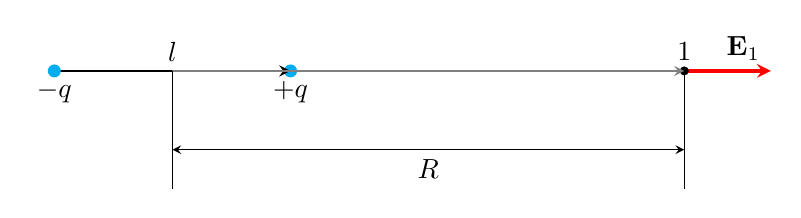
\begin{tikzpicture}[>=stealth]
	\draw[very thick, red, ->] (5, 0) -- (6.1, 0) node[black, above left] {$\textbf{E}_1$};
	\draw[cyan, fill] (0, 0) circle [radius=0.075];
	\draw[-latex, thick, ->] (-3, 0) node[below] {$-q$} -- (0, 0) node[below] {$+q$};
	\draw[cyan, fill] (-3, 0) circle [radius=0.075];
	\node[above] at (-1.5, 0) {$l$};

	\draw[fill] (5, 0) circle [radius=0.05];
	\draw[-latex, gray, semithick, ->] (-1.5, 0) -- (5, 0) node[black, above] {1};

	\draw[thin] (-1.5, 0) -- (-1.5, -1.5);
	\draw[thin] (5, 0) -- (5, -1.5);
	\draw[<->, thin] (-1.5, -1) -- (5, -1);
	\node[below] at (1.75, -1) {$R$};

\end{tikzpicture}
